\section{Workshops}
\label{workshops}

Vi gjennomførte i alt to workshops fordelt på to dager. Disse ble holdt på NSEP (Norsk senter for elektronisk pasientjournal) ved St. Olavs Hospital. Deltagerene var andreårs sykepleierstudenter ved HiST (Høyskolen i Sør-Trøndelag). En beskrivelse av hvordan gjennomføringen 

\begin{figure}[H]
\centering
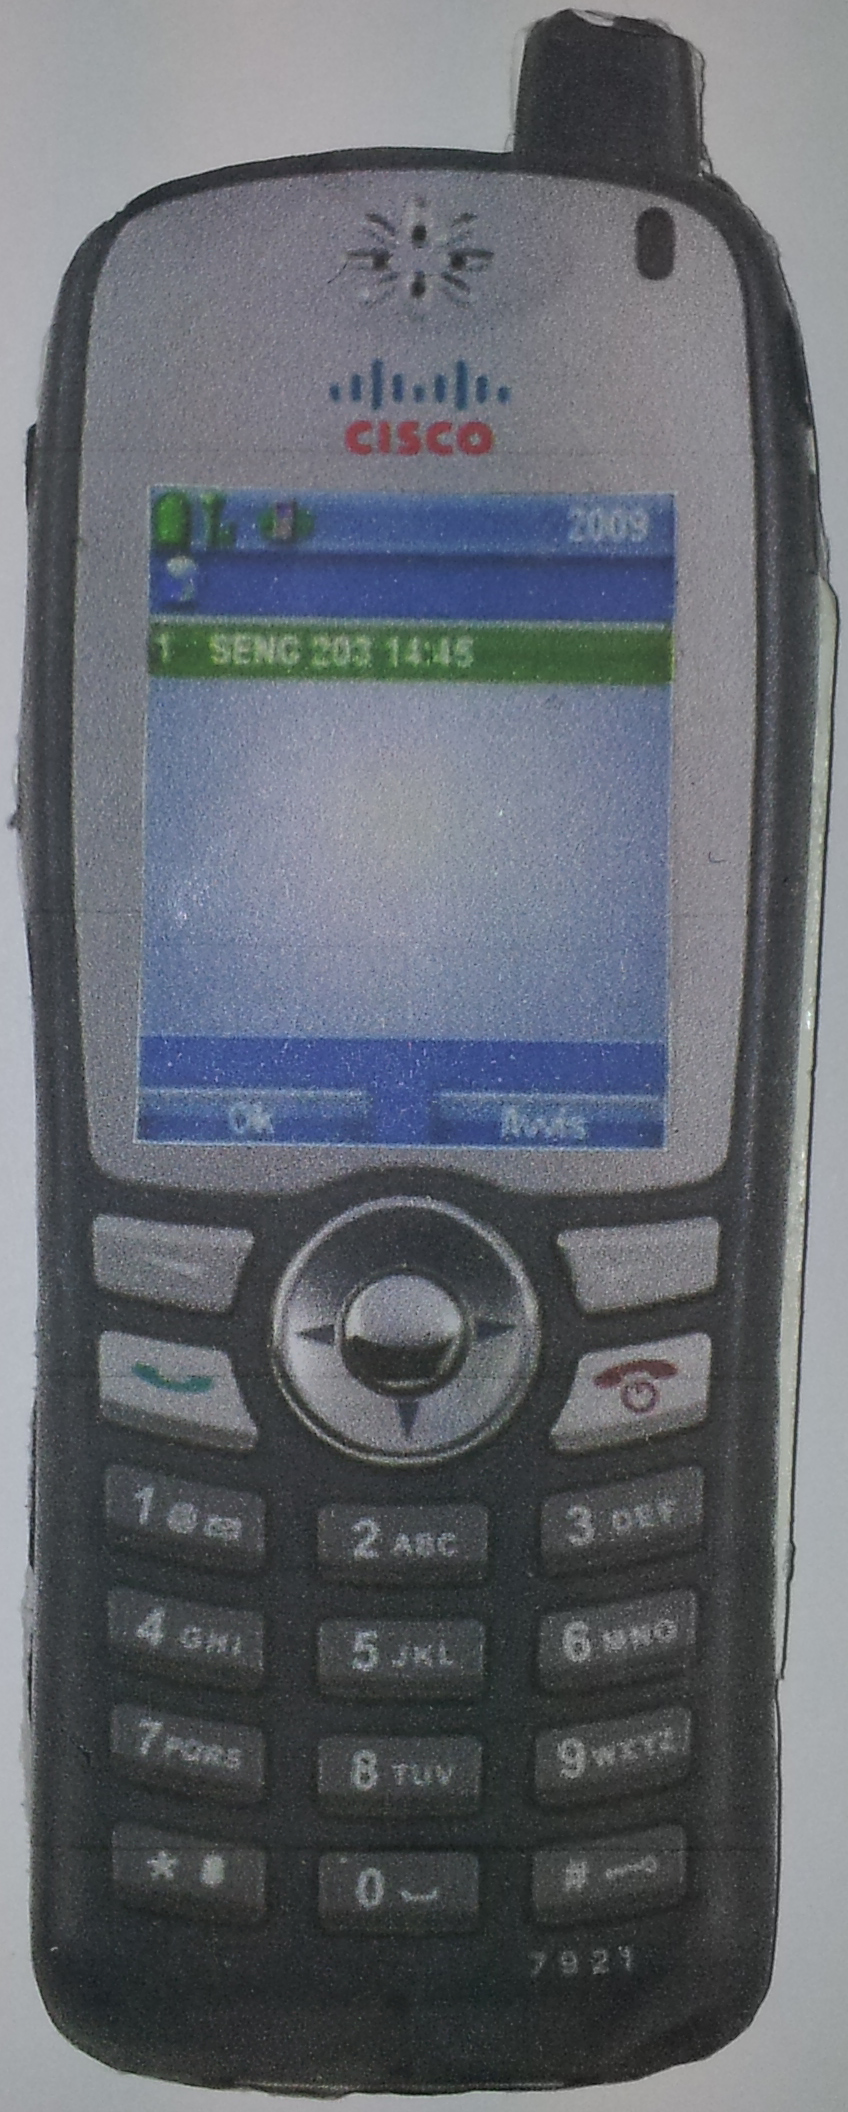
\includegraphics[scale=0.1]{mock-up_Telefon.jpg}
\caption{Mock-up av telefonen sykepleierene bruker i dag}
\label{mock-up_Telefon}
\end{figure}

\begin{figure}[H]
\centering
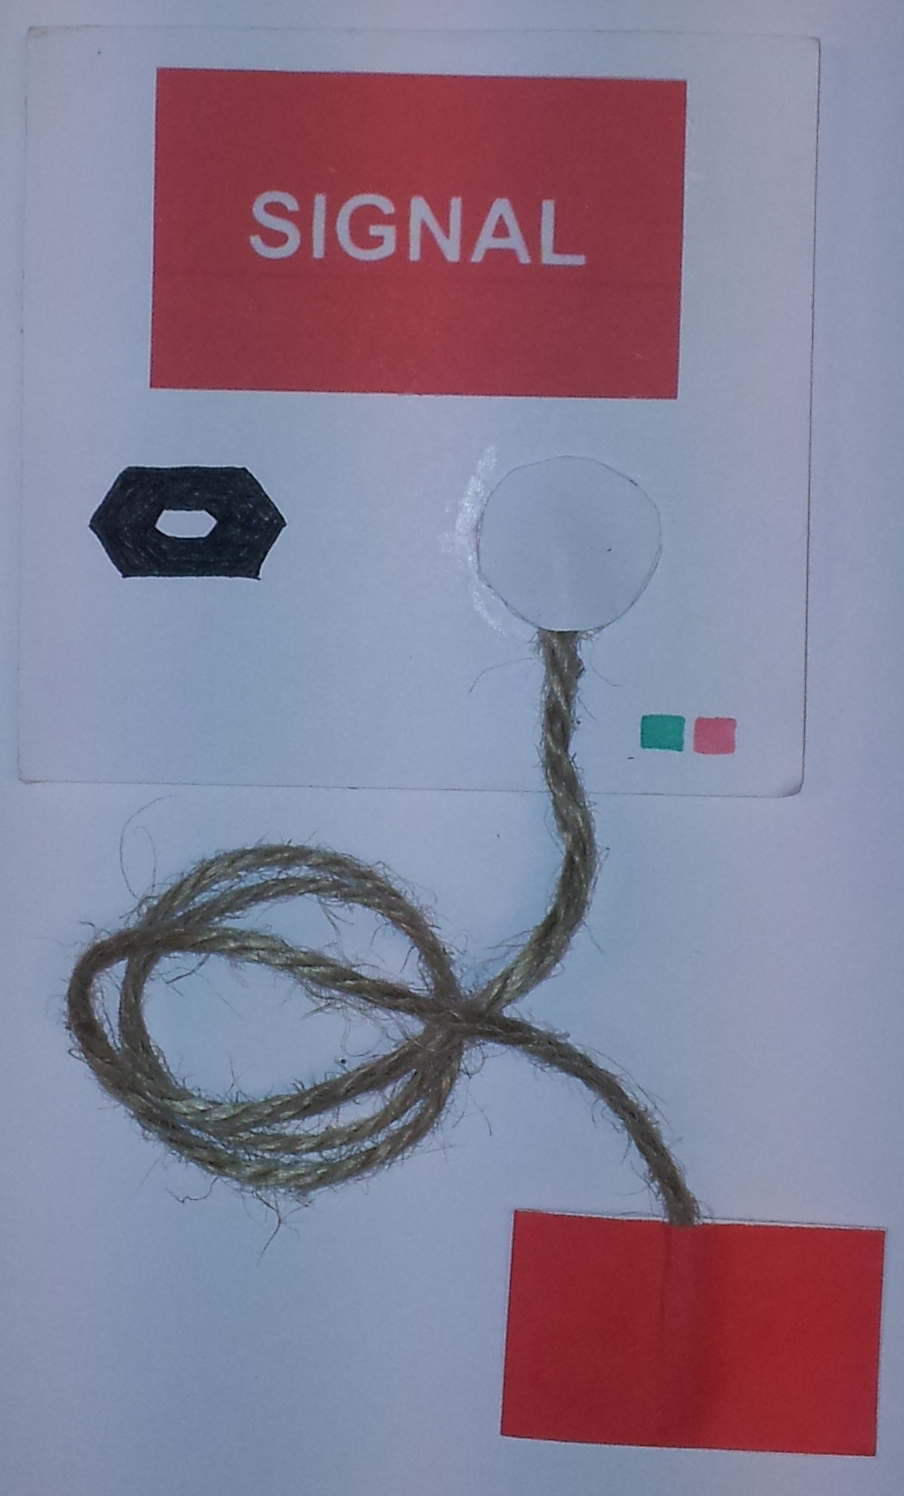
\includegraphics[scale=0.1]{mock-up_PasientPanel.jpg}
\caption{Mock-up av panelet hvor snoren pasienten kan trekke i er festet}
\label{mock-up_PasientPanel}
\end{figure}

\begin{figure}[H]
\centering
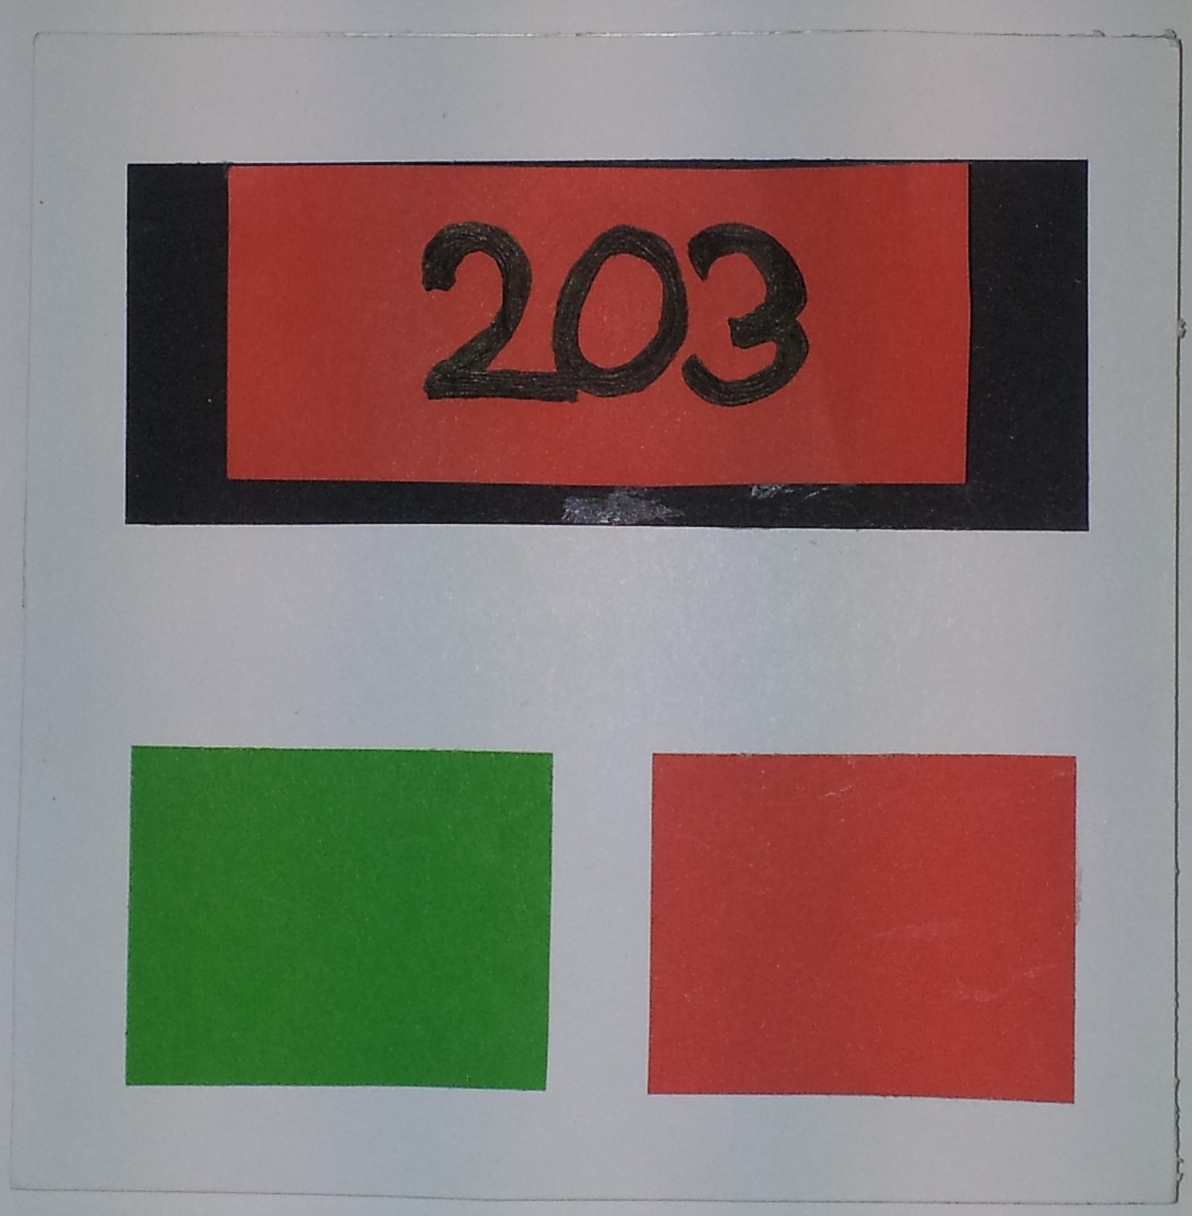
\includegraphics[scale=0.1]{mock-up_RomPanel.jpg}
\caption{Mock-up av panelet hvor sykepleiere trykker på den grønne knappen for å vise sin tilstedeværelse. Romnummer hvor pasientsignal er aktivt vil vises, her rom 203}
\label{mock-up_RomPanel}
\end{figure}

\begin{figure}[H]
\centering
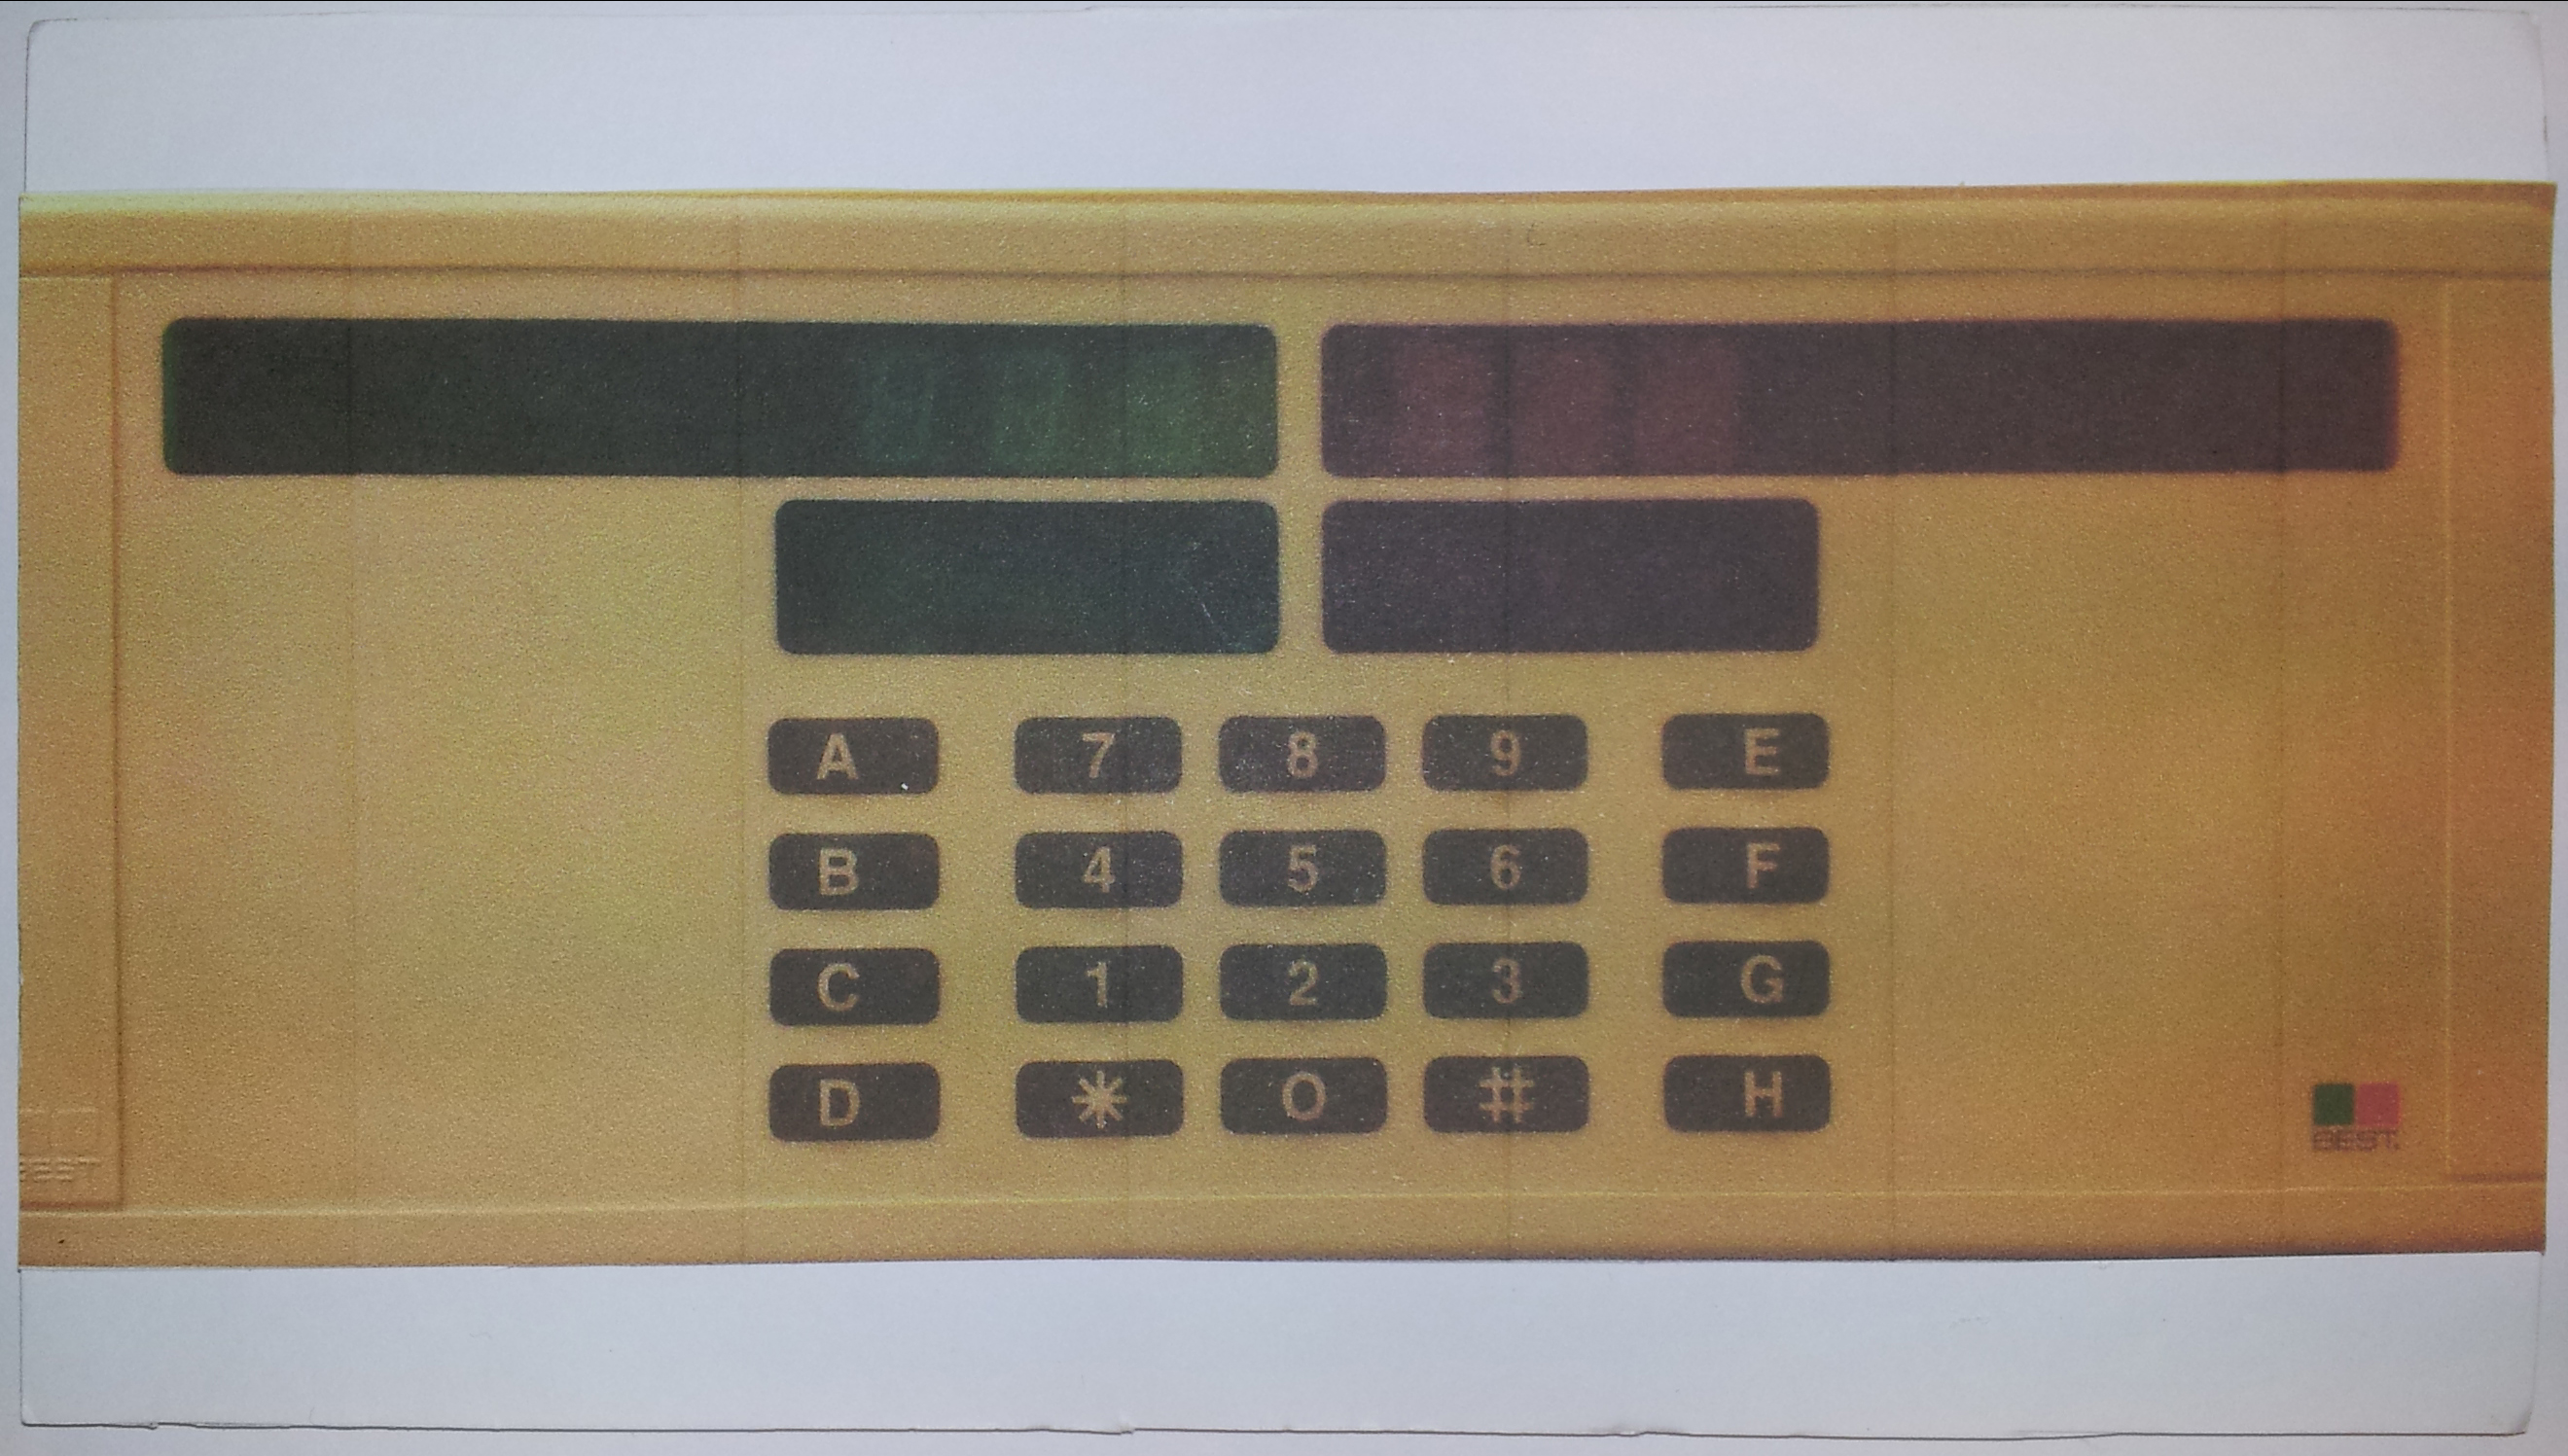
\includegraphics[scale=0.1]{mock-up_VaktPanel.jpg}
\caption{Mock-up av panelet plassert ved vaktposen på sengetunet. Her vises romnummer hvor pasientsignal er aktivt samt romnummer hvor sykepleiere har registrert tilstedeværelse}
\label{mock-up_VaktPanel}
\end{figure}